\appendix

\subsection{Liar’s Dice Rules and Game Mechanics}
\label{app:rules}

In the game, each player holds a private set of dice, while the dice of other players remain hidden. Game play consists of sequential bidding and challenges, with players reasoning probabilistically about unknown outcomes and strategically interpreting opponent actions.

\paragraph{\textbf{Players and Dice}}

The game consists of $N$ players. At the start of each round, each player is assigned $D$ fair six-sided dice, which are rolled privately. A player’s dice constitute their private information; the total number of dice in play is $N \times D$.

\paragraph{\textbf{Bidding Actions}}

Players take turns in a fixed order. On their turn, a player must either place a bid or challenge the most recent bid. A bid is an assertion $(q, f)$, where: $q \in N \times D$ is a quantity, $f \in \{1,2,3,4,5,6\}$ is a face value. The bid $(q, f)$ claims that among all dice in play, at least $q$ dice show face value $f$.

Bids must strictly increase according to a predefined ordering, prioritizing higher quantities and, secondarily, higher face values.

\paragraph{\textbf{Challenge Action}}

Instead of bidding higher, a player may challenge the most recent bid. When a bid $(q, f)$ is challenged, all dice from all players are revealed. If at least $q$ dice shows the face value $f$, the bid is valid; otherwise, it is invalid.

\paragraph{\textbf{Round Resolution and Payoffs}}

If the bid is valid, the challenger loses the round; if invalid, the bidder loses. The losing player forfeits one die, and a new round begins with all remaining dice re-rolled privately. The winner of the last round will be the first to bid in the next round.

\paragraph{\textbf{Game Termination}}

The game continues until only one player remains with at least one die. Since at most one die is lost per round and eliminating \(N-1\) players requires removing \(D\) dice from each, the game length is bounded below by \(D (N-1)\) rounds.

\paragraph{\textbf{Imperfect Information and Strategic Considerations}}

Because players observe only their own dice, Liar’s Dice requires reasoning over hidden information and opponent behavior. Bids convey both probabilistic claims and strategic intent, serving not only as stochastic signals about the game state but also as indicators of a player’s broader strategy.



\subsection{\textbf{Heuristic Agents}}
\label{app:heuristic_agents}

We implement a family of \emph{heuristic agents} that rely on simple, rule-based decision policies rather than explicit probabilistic inference. These agents serve as interpretable baselines and are designed to span a diverse space of bidding and challenge behaviors, isolating strategic dimensions such as risk tolerance, raise magnitude, belief approximation, and stochasticity.

\paragraph{\textbf{Common structure}}
All heuristic agents operate on the same observable information: the agent’s private dice, the current public bid, and the total number of dice in play. A bid \( b = (q,f) \) is treated as \emph{impossible} if its quantity exceeds the total number of dice; such bids are always challenged. Otherwise, agents choose between calling liar and producing a higher legal bid according to fixed rules.

\paragraph{\textbf{Conservative and aggressive bidding}}
At one extreme, the \emph{Conservative} agent challenges aggressively, calling liar whenever bids grow large and otherwise making minimal raises. At the other extreme, the \emph{Aggressive} agent prefers to continue bidding whenever possible, typically raising quantities and only calling liar when no legal raise remains. These agents model risk-averse and risk-seeking behaviors, respectively.

\paragraph{\textbf{Raise-preference heuristics}}
Several agents differ only in how they select among legal raises. \emph{Minimal-raise} agents always choose the smallest valid increase, while \emph{maximal-raise} agents choose the largest. These policies isolate the strategic effect of cautious versus forceful bidding without additional belief modeling.

\paragraph{\textbf{Frequency-based heuristics}}
Some agents exploit simple statistics of their private dice. For example, the \emph{MaxCount} agent opens by bidding the face it holds most frequently, while \emph{SafeFace} agents prefer bidding faces already present in hand. Variants such as \emph{Ones-Are-Wild} explicitly bias bids toward face \(1\) when wild-card rules apply.

\paragraph{\textbf{Threshold and expectation heuristics}}
Threshold-based agents call liar whenever the bid quantity exceeds a fixed or randomly chosen cutoff (e.g., half the total dice). The \emph{Probability} agent uses a crude expectation heuristic, comparing the bid quantity to the expected count \( D / |\mathcal{F}| \), where \( \mathcal{F} \) is the set of faces, without computing exact probabilities.

\paragraph{\textbf{Stochastic and adversarial behaviors}}
To increase behavioral diversity, we include agents that introduce randomness or non-standard logic, such as \emph{Bluffing} agents (occasionally bidding faces not in hand), \emph{Chaotic} agents (randomly choosing between raising and challenging), and pattern-based agents (e.g., parity- or cycle-based bidding).


\subsection{Approximate Nash Agent (Monte Carlo CFR)}
\label{app:mccfr_agent}

To approximate equilibrium play, we implement a Nash-style agent based on \emph{External Sampling Monte Carlo Counterfactual Regret Minimization} (MCCFR)\cite{mccfr}. This agent represents a game-theoretic baseline beyond heuristic or myopic strategies, as it approximates a Nash equilibrium in extensive-form games.

\paragraph{\textbf{Game model and information sets}}
The agent models Liar’s Dice as an extensive-form game with imperfect information. An information set is defined as
\[
I = (d_{\text{me}}, q_{\text{last}}, f_{\text{last}}),
\]
where \( d_{\text{me}} \) denotes the agent’s private dice (sorted), and \( (q_{\text{last}}, f_{\text{last}}) \) denotes the most recent public bid (or \texttt{None} at the start of the game). The agent does not observe opponent dice, only their aggregate count.

\paragraph{Policy representation.}
For each dice configuration and face set, the learned strategy is stored as a policy
\[
\pi_I(a) \in [0,1],
\quad \sum_{a \in A(I)} \pi_I(a) = 1,
\]
where \( A(I) \) is the set of legal actions at information set \( I \), consisting of all valid higher bids and the action \texttt{call\_liar}. At inference time, actions are sampled according to the learned distribution \( \pi_I \).

\paragraph{\textbf{Training via MCCFR}}
Training is performed offline using external-sampling MCCFR. At each iteration:
\begin{enumerate}
    \item Dice outcomes for all players are sampled (chance sampling).
    \item One player is designated as the traversing player.
    \item For traversing nodes, all actions are explored to update counterfactual regrets.
    \item For opponent nodes, a single action is sampled according to the current strategy.
\end{enumerate}

Regret matching is used to derive strategies from cumulative regrets. Let
\[
Z_I = \sum_{a'} \max(R_I(a'), 0).
\]
Then
\[
\pi_I(a) =
\begin{cases}
\dfrac{\max(R_I(a), 0)}{Z_I}, & \text{if } Z_I > 0, \\ \\
\dfrac{1}{|A(I)|}, & \text{otherwise}.
\end{cases}
\]

\paragraph{\textbf{Utility definition}}
Terminal utilities are assigned only when a \texttt{call\_liar} action occurs. Let \( b = (q,f) \) be the last bid. If the bid is true, the caller receives utility \(-1\); otherwise, the caller receives \(+1\). Utilities are zero-sum between players.

\paragraph{\textbf{Convergence monitoring}}
Optionally, the algorithm tracks convergence by measuring the maximum change in strategy probabilities across sampled information sets. Training halts early if this change falls below a predefined threshold.

\paragraph{\textbf{Deployment and fallback policy}}
At runtime, the agent loads pre-trained policies indexed by dice-count configurations. If no matching policy is found, the agent \textbf{fallback} to selecting a random legal action. This agent is limited to our game configurations, as changes in maximal dice count, players or rules may expose new states the agent was not trained on and skew regrets.

\paragraph{\textbf{Training configuration}}
The MCCFR agent is trained offline using external-sampling Monte Carlo CFR for a fixed dice configuration. Training proceeds for a maximum of $10{,}000$ iterations, unless early convergence is detected. At each iteration, a full chance sample of player dice is drawn, and two traversal passes are executed, one for each player as the traversing player.

Optionally, convergence is monitored by tracking changes in the agent’s average strategy. Every $500$ iterations, the normalized action probabilities derived from the accumulated strategy sums are compared against a stored snapshot from the previous checkpoint. Convergence is declared when the maximum absolute change in action probability across a sampled subset of information sets falls below a threshold of $0.001$, at which point training terminates early.

This criterion reflects empirical stabilization of the learned policy rather than formal exploitability bounds, and is used to prevent unnecessary additional sampling once the strategy distribution ceases to change meaningfully.
\subsection{Supplementary Result Tables and Figures}
\label{app:supplementary_results}

This section preserves the detailed result material omitted from the compact workshop submission. The main paper reports condensed summaries; the tables and figures here provide the fuller diagnostics used to support those summaries.

\paragraph{Policy-level PPO--MCCFR comparisons.}
Figures~\ref{fig:app_mccfr_call_liar}--\ref{fig:app_mccfr_opening} report the call-liar and opening-bid distributions used to compare the population-trained PPO policy against the MCCFR baseline.

\begin{figure}[t]
    \centering
    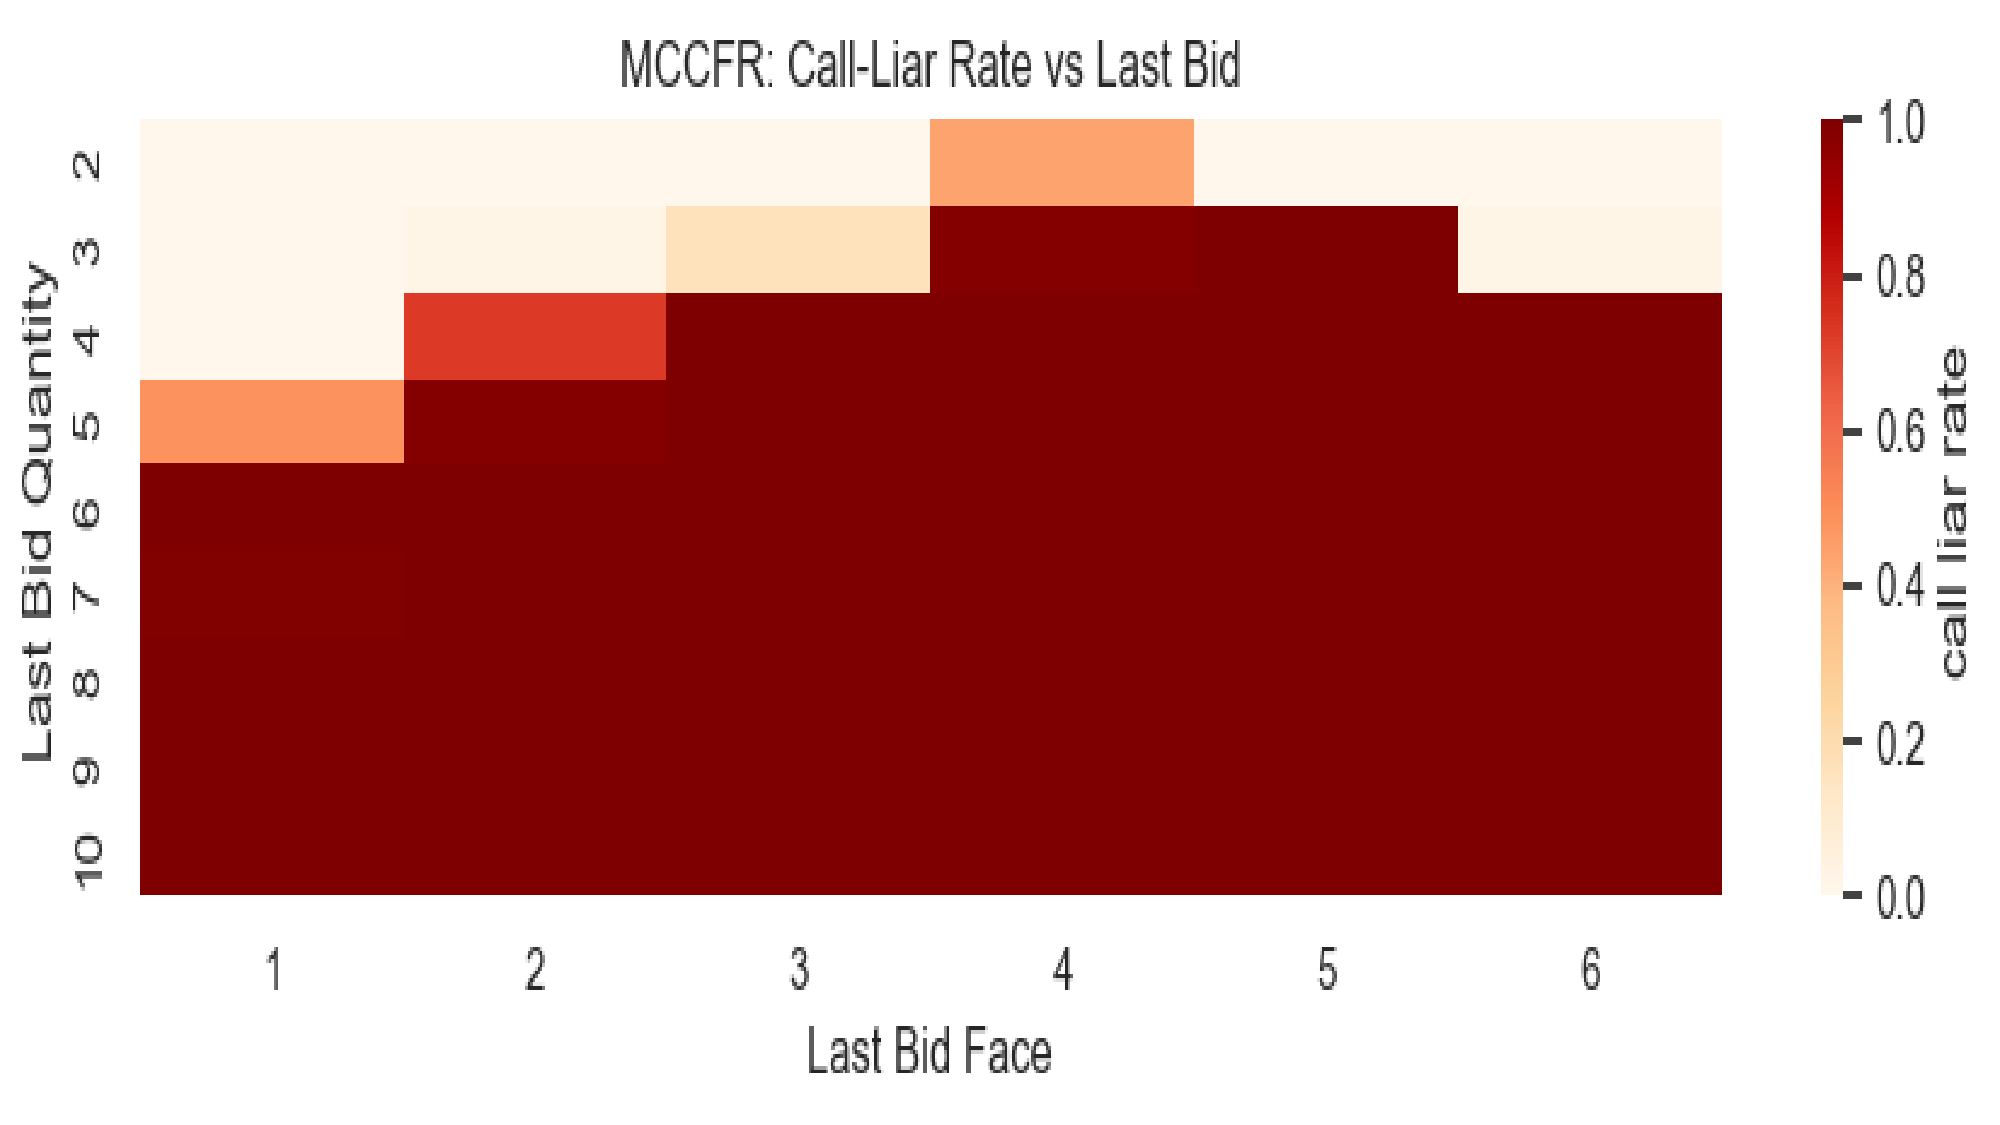
\includegraphics[width=\columnwidth]{images/call_liar_mccfr.pdf}
    \caption{MCCFR call-liar rate as a function of the opponent's last bid quantity and face.}
    \label{fig:app_mccfr_call_liar}
\end{figure}

\begin{figure}[t]
    \centering
    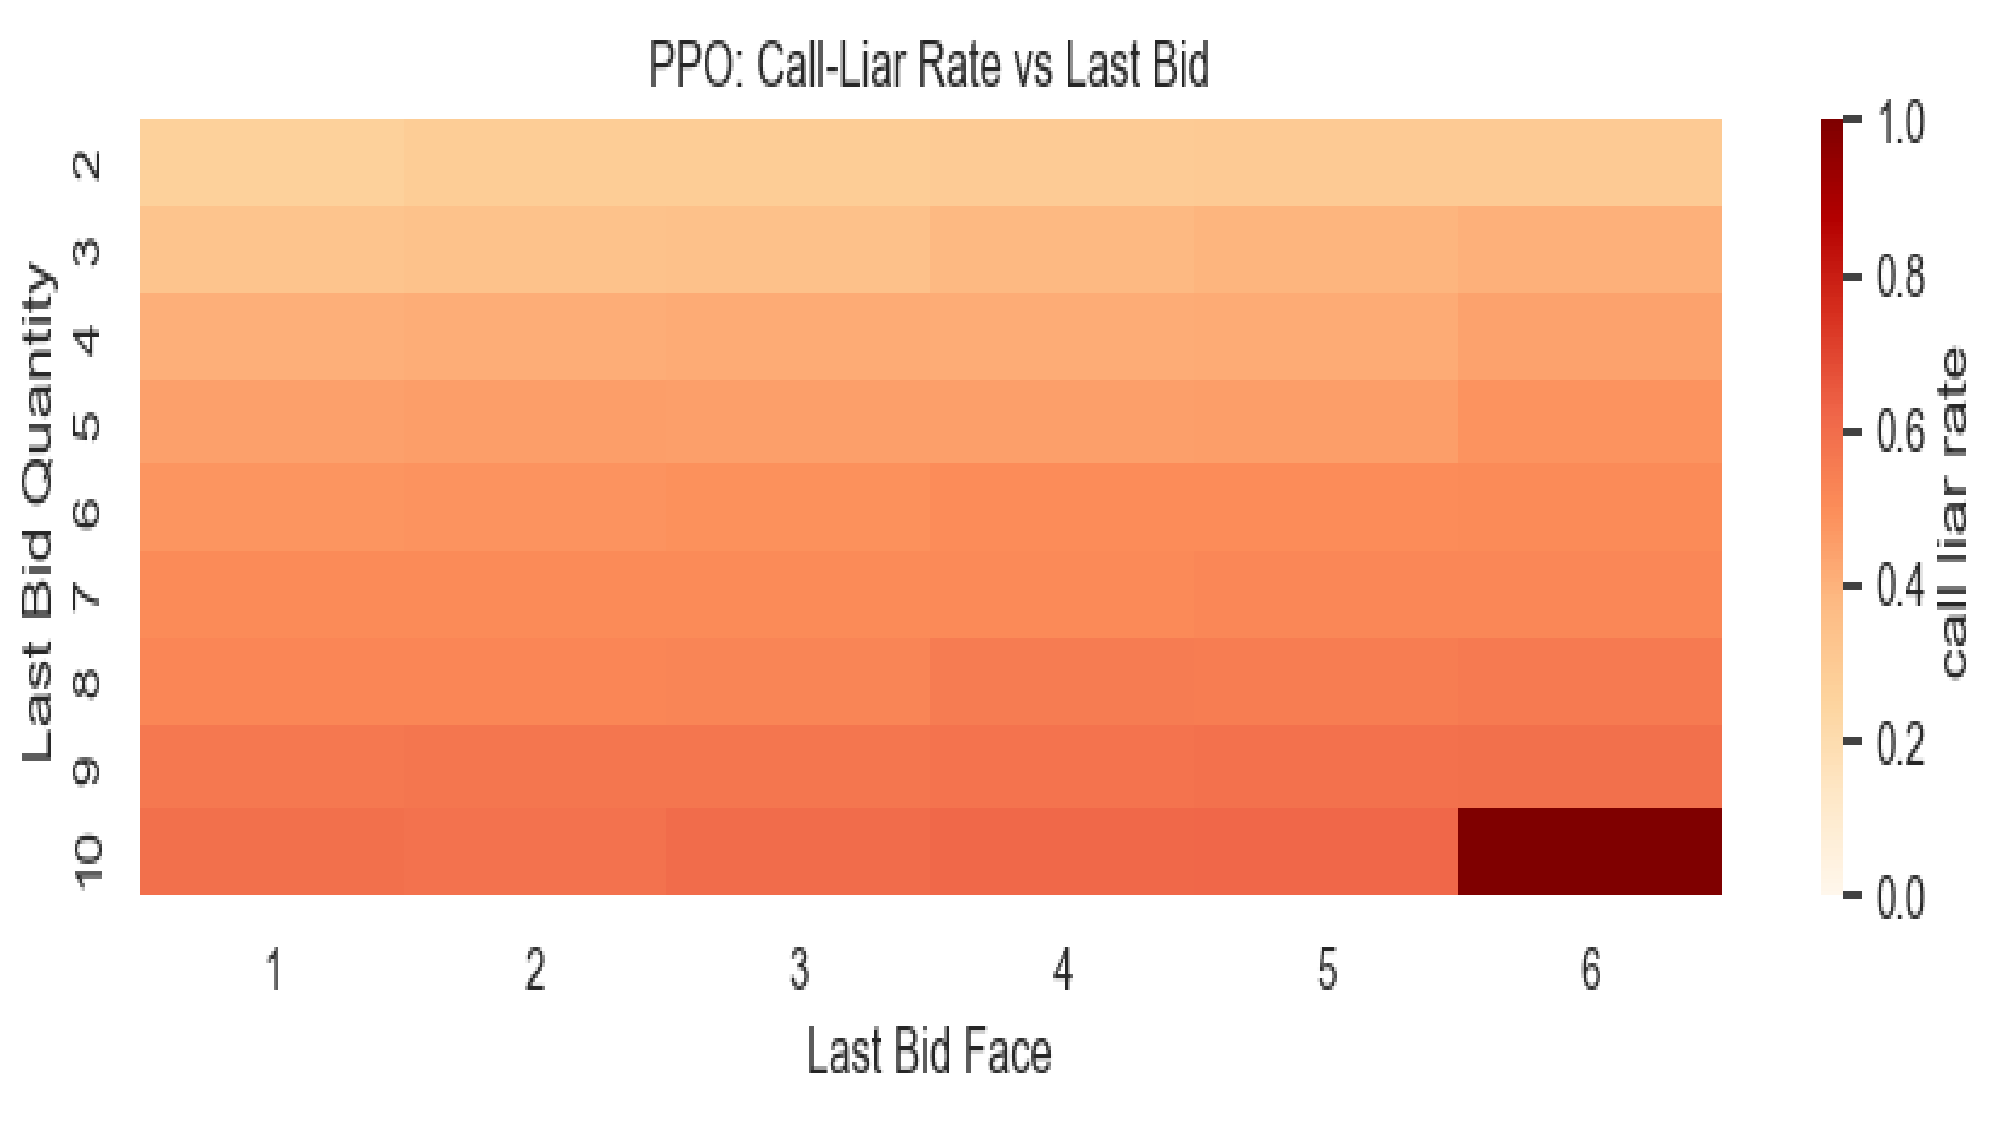
\includegraphics[width=\columnwidth]{images/call_liar_ppo.pdf}
    \caption{PPO call-liar rate as a function of the opponent's last bid quantity and face.}
    \label{fig:app_ppo_call_liar}
\end{figure}

\begin{figure}[t]
    \centering
    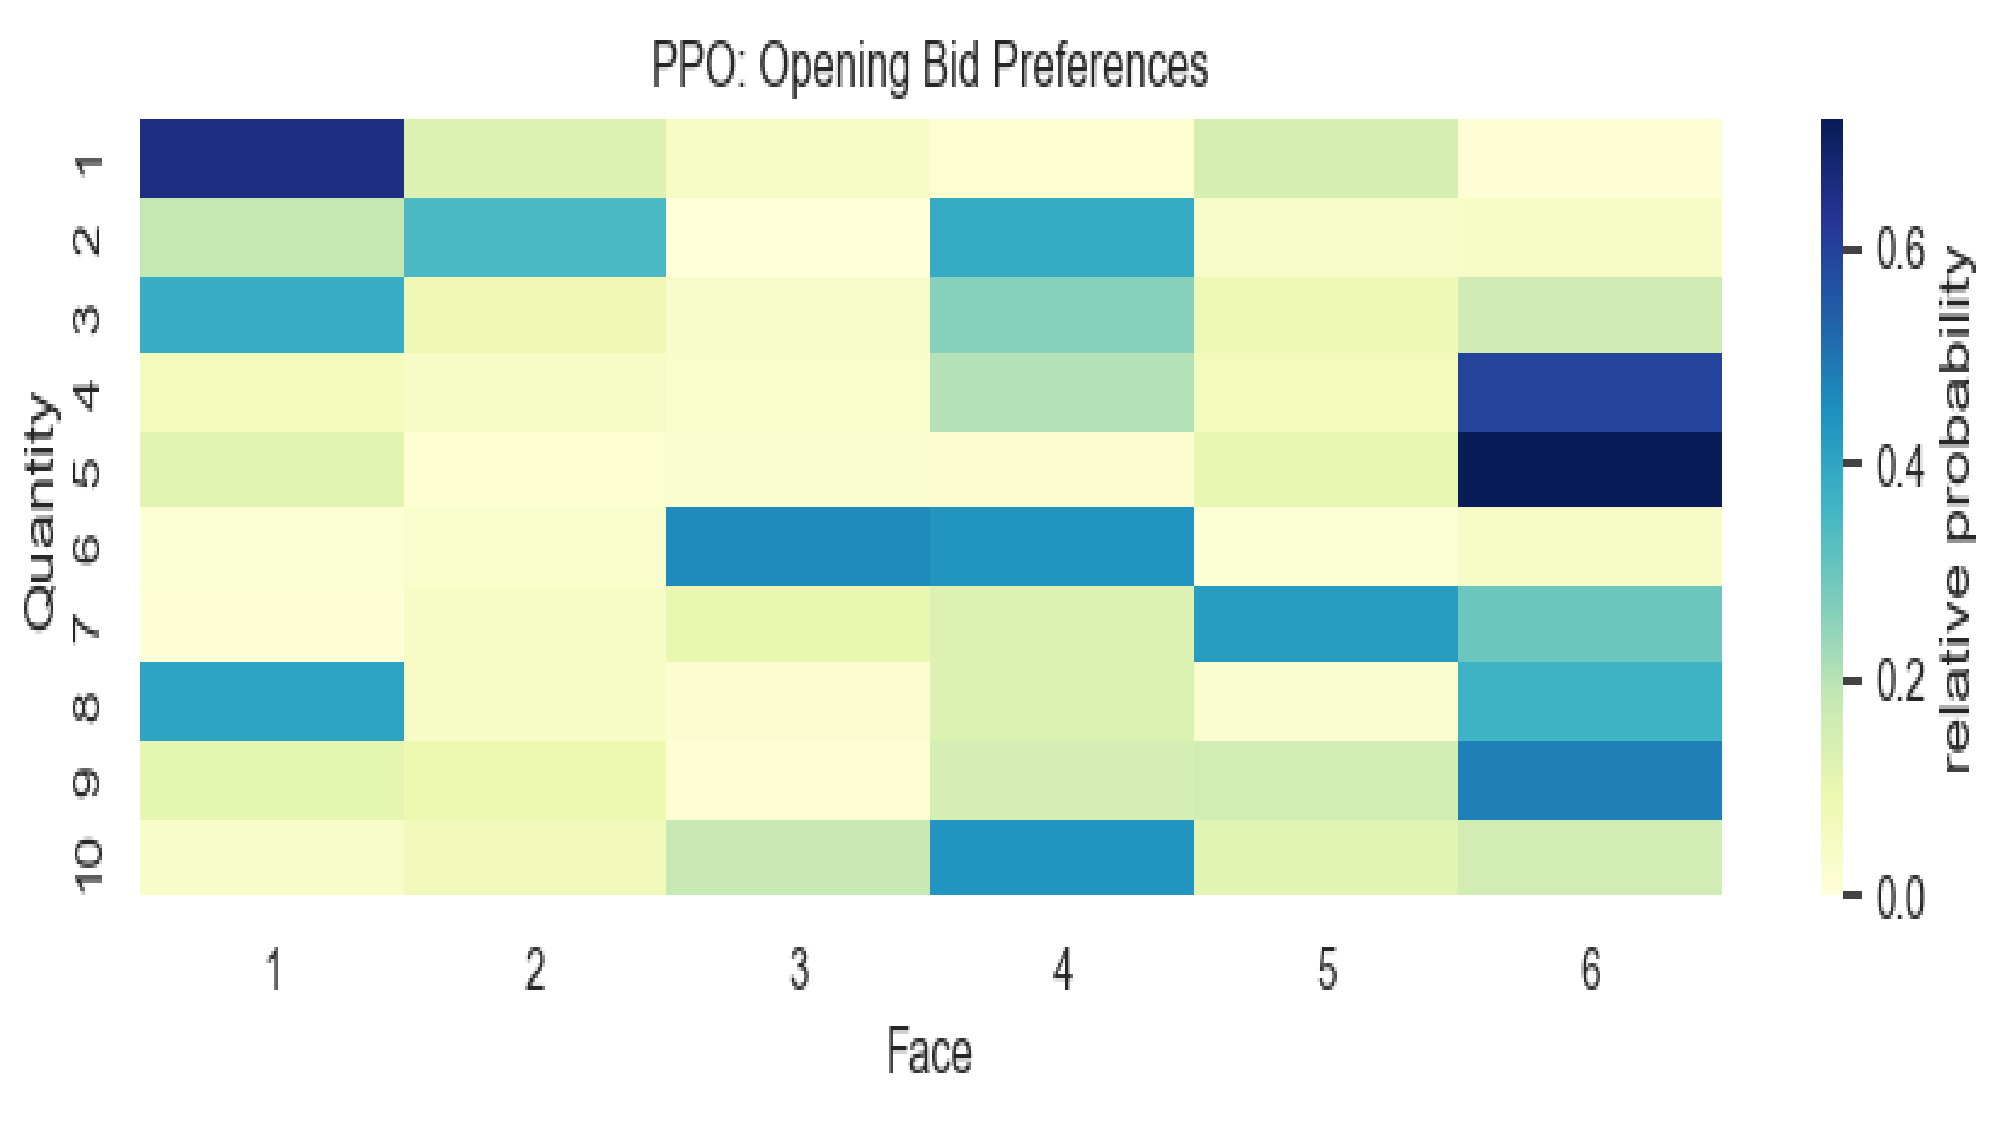
\includegraphics[width=\columnwidth, trim=0cm 4cm 0cm 0cm,clip]{images/opening_bid_preference_ppo.pdf}
    \caption{Opening bid preferences of the PPO agent.}
    \label{fig:app_ppo_opening}
\end{figure}

\begin{figure}[t]
    \centering
    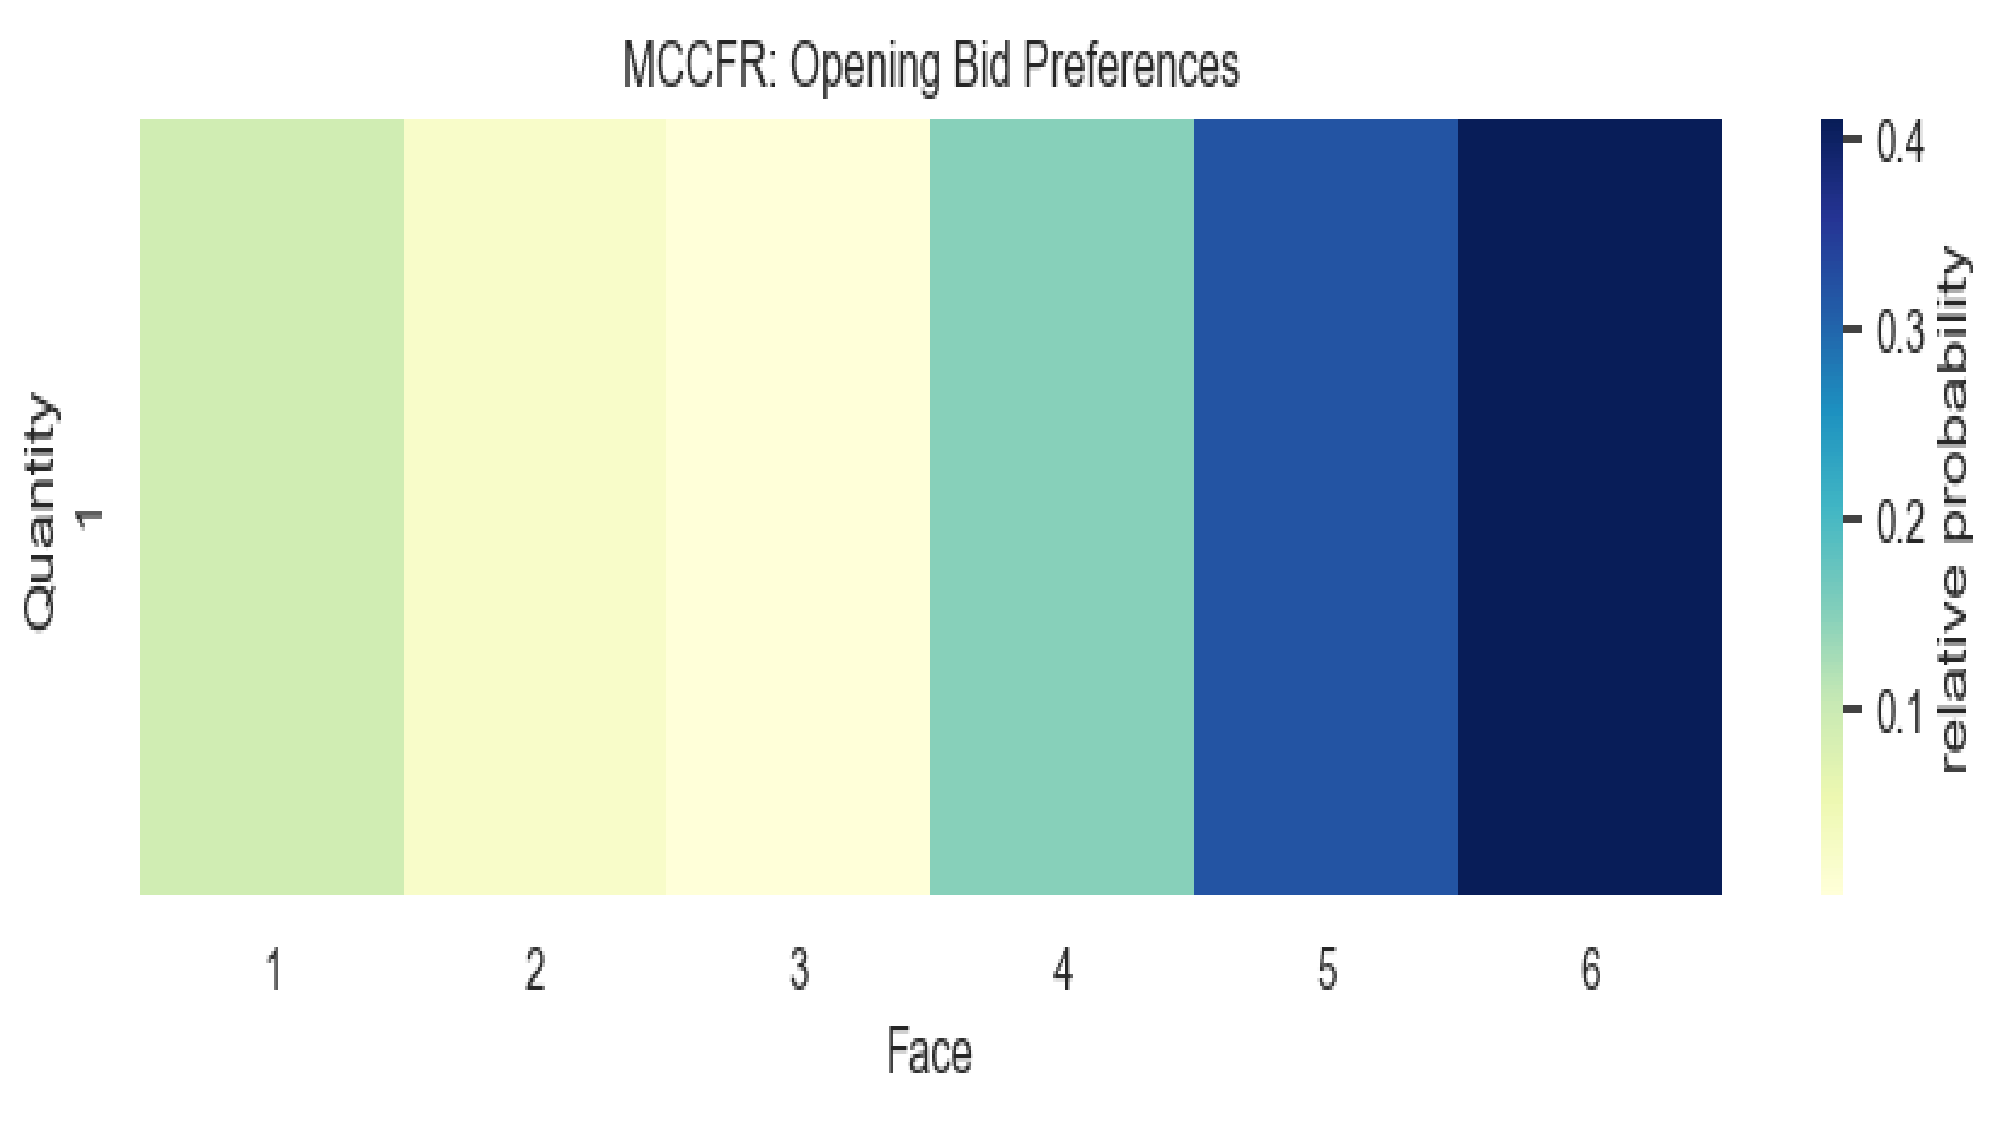
\includegraphics[width=\columnwidth, trim=0cm 4cm 0cm 0cm,clip]{images/opening_bid_preference_mccfr.pdf}
    \caption{Opening bid preferences of the MCCFR agent.}
    \label{fig:app_mccfr_opening}
\end{figure}

\paragraph{Full non-adaptive tournament table.}
Table~\ref{tab:app_agent_behavior_statistics} reports the full static-agent tournament table that was condensed in the main paper.

\begin{table}[t]
\centering
\scriptsize
\resizebox{\columnwidth}{!}{%
\begin{tabular}{lccccc}
\toprule
Agent & Win \% & Avg. steps & Avg. bids & Avg. calls & Avg. bluffs \\
\midrule
\textbf{RL (PPO)} & \textbf{93.14\%} & 19.95 & 13.85 & 6.10 & 5.73 \\
Bayesian & 92.36\% & 22.41 & 16.81 & 5.59 & 4.10 \\
ProbabilityMinRaise & 81.93\% & 36.34 & 30.25 & 6.10 & 4.69 \\
ThresholdLiar & 71.31\% & 47.09 & 41.50 & 5.59 & 4.95 \\
MaxCount & 69.17\% & 26.04 & 20.38 & 5.65 & 4.75 \\
Parity & 67.88\% & 29.05 & 22.58 & 6.47 & 4.24 \\
RandomThreshold & 65.70\% & 45.88 & 40.39 & 5.49 & 4.86 \\
Conservative & 62.71\% & 46.44 & 40.99 & 5.45 & 4.88 \\
CycleFace & 62.42\% & 50.38 & 44.77 & 5.60 & 5.01 \\
Alternator & 62.31\% & 22.16 & 15.16 & 7.00 & 3.81 \\
MinRaise & 62.02\% & 46.47 & 41.02 & 5.45 & 4.85 \\
Mirror & 56.54\% & 30.52 & 24.75 & 5.77 & 5.15 \\
Bluffing & 54.52\% & 40.56 & 34.89 & 5.66 & 4.82 \\
OnesAreWild & 49.98\% & 38.33 & 32.74 & 5.59 & 4.69 \\
SafeFace & 49.82\% & 38.36 & 32.77 & 5.59 & 4.70 \\
NashCFR & 45.42\% & 37.61 & 31.68 & 5.93 & 5.16 \\
RandomFace & 29.48\% & 20.34 & 14.81 & 5.53 & 5.23 \\
ProbabilityMaxRaise & 24.77\% & 16.61 & 11.04 & 5.57 & 5.05 \\
Chaotic & 21.71\% & 18.93 & 12.79 & 6.14 & 4.68 \\
ChaoticSafe & 21.61\% & 18.94 & 12.79 & 6.15 & 4.69 \\
Aggressive & 17.53\% & 16.07 & 10.72 & 5.35 & 5.31 \\
MaxRaise & 17.26\% & 16.40 & 11.06 & 5.35 & 5.15 \\
ChaoticUnsafe & 13.22\% & 19.34 & 13.21 & 6.12 & 4.66 \\
\bottomrule
\end{tabular}}
\caption{Overall win rates in the non-adaptive agent-versus-agent tournament with high-level behavioral statistics.}
\label{tab:app_agent_behavior_statistics}
\end{table}

\begin{figure*}[t]
    \centering
    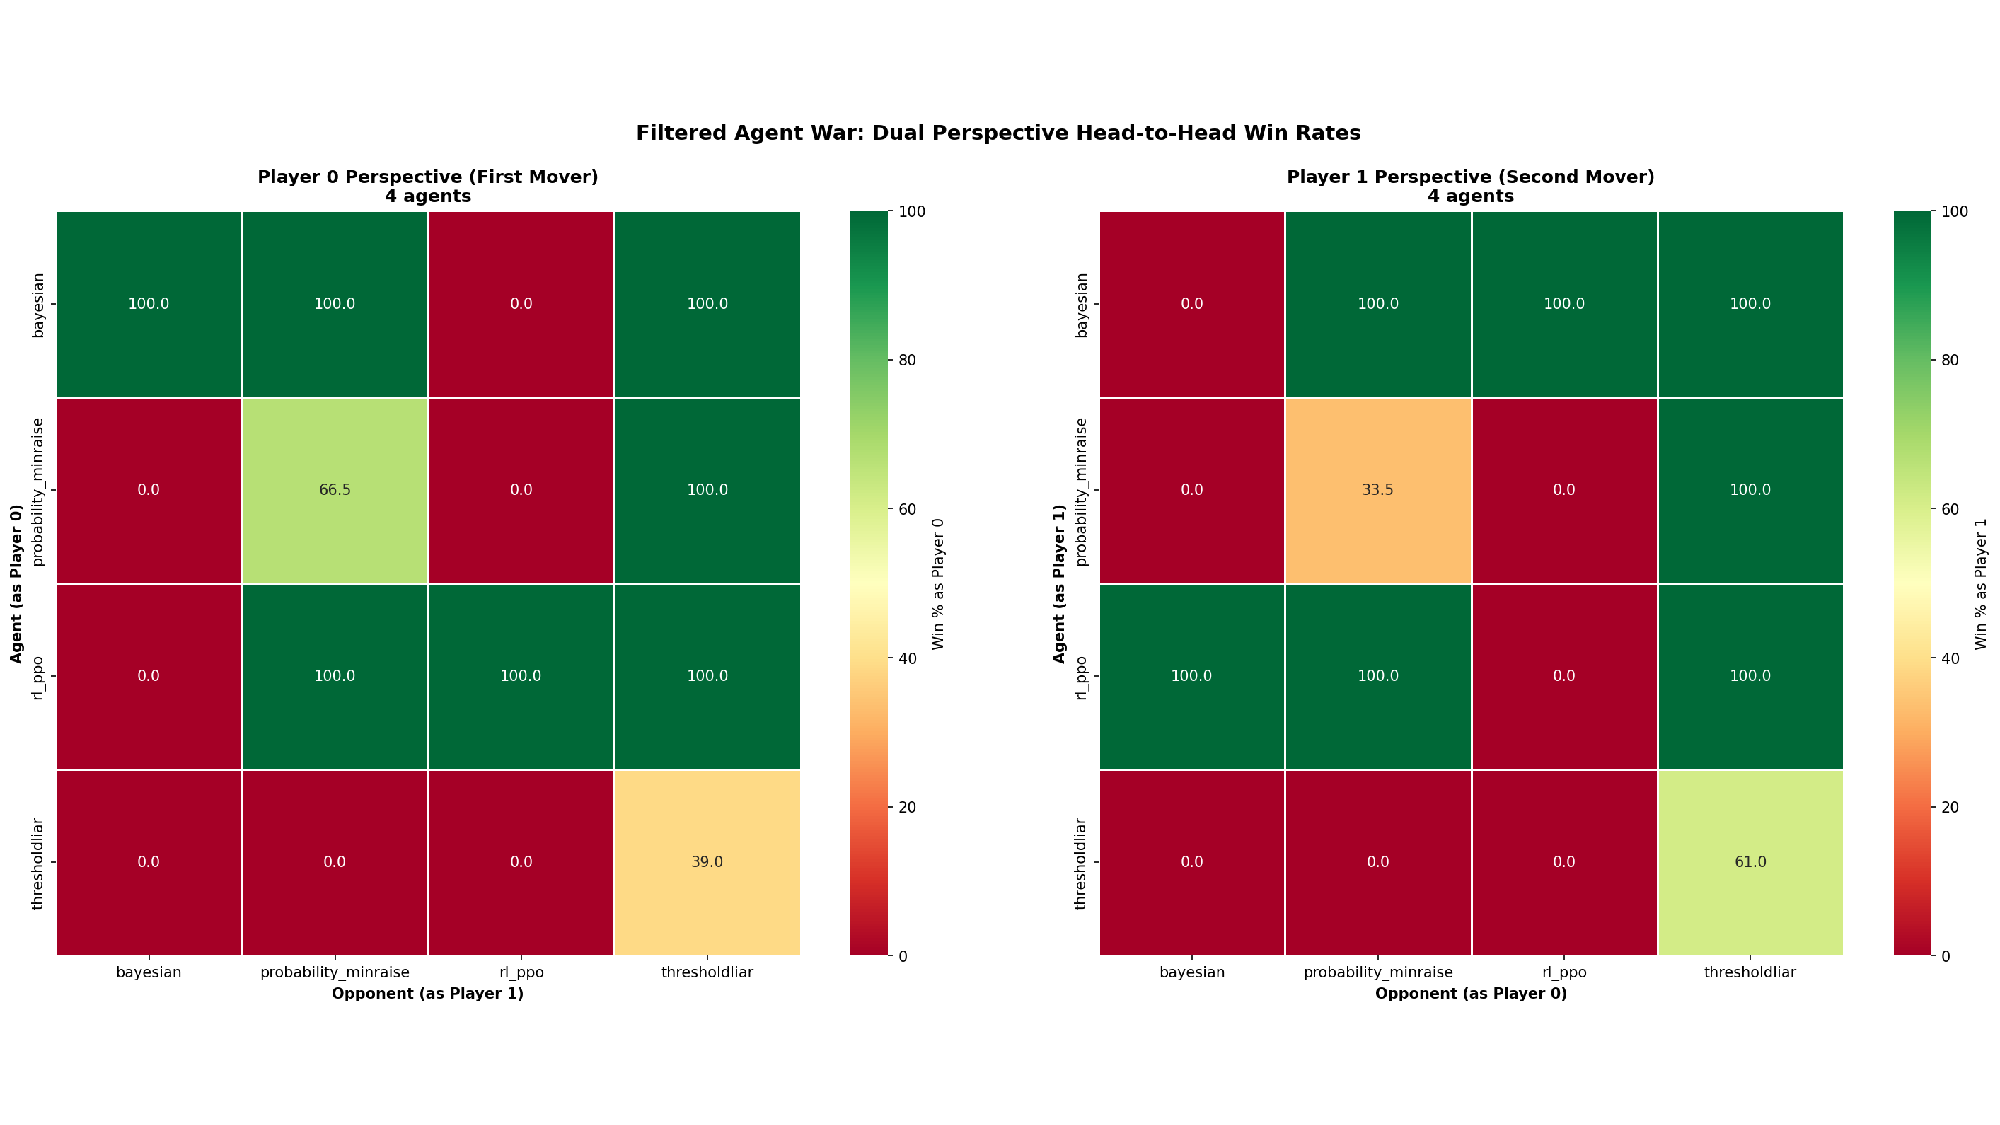
\includegraphics[width=\textwidth, trim=0cm 2cm 0cm 0cm,clip]{images/head_to_head_top_4.pdf}
    \caption{Dual-perspective head-to-head win rates for the top-performing agents. Each cell reports win rates when the row agent plays as Player~0 (first mover, left) or Player~1 (second mover, right).}
    \label{fig:app_head_to_head_top_4}
\end{figure*}

\paragraph{Adaptive-agent identification and per-opponent performance.}
Tables~\ref{tab:app_adaptive_identification} and~\ref{tab:app_adaptive_winrates} provide detailed adaptive-agent results by opponent type.

\begin{table}[t]
\centering
\scriptsize
\begin{tabular}{lcc}
\toprule
Opponent & Accuracy & Mean steps to ID \\
\midrule
AggressiveAgent & 100.0\% & $3.10 \pm 0.94$ \\
BayesianAgent & 100.0\% & $2.00 \pm 0.00$ \\
MaxRaiseAgent & 100.0\% & $3.00 \pm 1.00$ \\
RandomFaceAgent & 93.0\% & $3.00 \pm 1.00$ \\
NashCFRAgent & 92.5\% & $2.00 \pm 0.00$ \\
MirrorAgent & 72.0\% & $3.39 \pm 0.92$ \\
BluffingAgent & 69.5\% & $2.98 \pm 1.00$ \\
MaxCountBidAgent & 50.0\% & $2.00 \pm 0.00$ \\
GeneralistPPO & 50.0\% & $3.00 \pm 0.00$ \\
SafeFaceAgent & 50.0\% & $4.00 \pm 0.00$ \\
ConservativeAgent & 50.0\% & $2.00 \pm 0.00$ \\
CycleFaceAgent & 50.0\% & $2.00 \pm 0.00$ \\
RandomThresholdAgent & 46.5\% & $3.89 \pm 0.45$ \\
ChaoticSafeAgent & 39.0\% & $3.00 \pm 0.88$ \\
ChaoticUnsafeAgent & 36.0\% & $3.03 \pm 0.73$ \\
AlternatorAgent & 26.5\% & $2.00 \pm 0.00$ \\
ChaoticAgent & 19.0\% & $2.95 \pm 0.79$ \\
ThresholdLiarAgent & 18.5\% & $2.00 \pm 0.00$ \\
ProbabilityMinRaiseAgent & 18.0\% & $2.00 \pm 0.00$ \\
MinRaiseAgent & 10.5\% & $2.00 \pm 0.00$ \\
ProbabilityMaxRaiseAgent & 1.5\% & $2.00 \pm 0.00$ \\
\midrule
OnesAreWildAgent & 0.0\% & -- \\
ParityAgent & 0.0\% & -- \\
\bottomrule
\end{tabular}
\caption{Opponent identification accuracy and mean number of steps to correct identification, reported for games in which identification was correct.}
\label{tab:app_adaptive_identification}
\end{table}

\begin{table}[t]
\centering
\scriptsize
\resizebox{\columnwidth}{!}{%
\begin{tabular}{lccc}
\toprule
Opponent & Win \% & $WR_{P0}$ & $WR_{P1}$ \\
\midrule
AggressiveAgent & 100\% & 100\% & 100\% \\
BluffingAgent & 100\% & 100\% & 100\% \\
BayesianAgent & 100\% & 100\% & 100\% \\
FaceFixedRandomAgent & 100\% & 100\% & 100\% \\
CautiousRandomAgent & 100\% & 100\% & 100\% \\
FaceRandomRandomAgent & 100\% & 100\% & 100\% \\
ConservativeAgent & 100\% & 100\% & 100\% \\
CycleFaceAgent & 100\% & 100\% & 100\% \\
MinRaiseAgent & 100\% & 100\% & 100\% \\
MaxRaiseAgent & 100\% & 100\% & 100\% \\
MaxCountBidAgent & 100\% & 100\% & 100\% \\
GeneralistPPO & 100\% & 100\% & 100\% \\
ParityAgent & 100\% & 100\% & 100\% \\
RandomAgent & 100\% & 100\% & 100\% \\
RandomThresholdAgent & 100\% & 100\% & 100\% \\
RandomFaceAgent & 100\% & 100\% & 100\% \\
SafeFaceAgent & 100\% & 100\% & 100\% \\
MirrorAgent & 100\% & 100\% & 100\% \\
NashCFRAgent & 100\% & 100\% & 100\% \\
OnesAreWildAgent & 100\% & 100\% & 100\% \\
ThresholdLiarAgent & 100\% & 100\% & 100\% \\
\midrule
ChaoticAgent & 99\% & 100\% & 99\% \\
ChaoticUnsafeAgent & 99\% & 99\% & 100\% \\
AggressiveRandomAgent & 99\% & 98\% & 100\% \\
ChaoticSafeAgent & 99\% & 100\% & 98\% \\
ProbabilityMaxRaiseAgent & 96\% & 92\% & 100\% \\
ProbabilityMinRaiseAgent & 90\% & 80\% & 100\% \\
AlternatorAgent & 53\% & 48\% & 58\% \\
\bottomrule
\end{tabular}}
\caption{Win rates of the adaptive agent against each opponent, overall and by player position (P0: first mover, P1: second mover).}
\label{tab:app_adaptive_winrates}
\end{table}

\paragraph{Additional diagnostics.}
Tables~\ref{tab:app_latency_analysis}--\ref{tab:app_multi_agent_results} preserve the latency, correlation, and multi-agent transfer diagnostics omitted from the compact main paper.

\begin{table}[t]
\centering
\scriptsize
\begin{tabular}{lc}
\toprule
Agent & Time per turn (ms) \\
\midrule
Bayesian & $0.014 \pm 0.012$ \\
Conservative & $0.005 \pm 0.004$ \\
Nash (CFR) & $0.008 \pm 0.011$ \\
RL (PPO) & $0.570 \pm 1.971$ \\
Adaptive Agent & $0.741 \pm 0.843$ \\
\bottomrule
\end{tabular}
\caption{Agent decision time per turn, reported as mean $\pm$ standard deviation.}
\label{tab:app_latency_analysis}
\end{table}

\begin{table}[t]
\centering
\scriptsize
\resizebox{\columnwidth}{!}{%
\begin{tabular}{lccccc}
\toprule
 & Win \% & Avg. steps & Avg. bids & Avg. calls & Avg. bluffs \\
\midrule
Win \%        & - & 0.48 & 0.47 & 0.17 & 0.12 \\
Avg. steps   & - & - & 0.999 & 0.26 & 0.01 \\
Avg. bids    & - & - & - & 0.29 & 0.03 \\
Avg. calls   & - & - & - & - & 0.51 \\
Avg. bluffs  & - & - & - & - & - \\
\bottomrule
\end{tabular}}
\caption{Pearson correlation matrix between win rate and behavioral statistics.}
\label{tab:app_correlation_matrix}
\end{table}

\begin{table}[t]
\scriptsize
\centering
\begin{tabular}{llccc}
\toprule
Game setting & Agent & Wins & Win\% & Avg turns \\
\midrule
\multirow{3}{*}{3 agents (heuristics)}
 & \textbf{Bayesian} & \textbf{991} & \textbf{99.1} & 30.0 \\
 & Conservative & 9 & 0.9 & 24.7 \\
 & Probability MaxRaise & 0 & 0.0 & 9.3 \\
\midrule
\multirow{3}{*}{3 agents (with PPO)}
 & \textbf{Bayesian} & \textbf{947} & \textbf{94.7} & 24.9 \\
 & Conservative & 50 & 5.0 & 20.9 \\
 & RL (PPO) & 3 & 0.3 & 13.6 \\
\midrule
\multirow{4}{*}{4 agents}
 & \textbf{Bayesian} & \textbf{887} & \textbf{88.7} & 24.2 \\
 & Conservative & 94 & 9.4 & 21.5 \\
 & Probability MaxRaise & 0 & 0.0 & 10.5 \\
 & RL (PPO) & 19 & 1.9 & 20.0 \\
\bottomrule
\end{tabular}
\caption{Results of 1{,}000 multi-agent Liar's Dice games across different agent configurations.}
\label{tab:app_multi_agent_results}
\end{table}


